\documentclass[12pt,a4paper]{article}

\usepackage[a4paper,text={16.5cm,25.2cm},centering]{geometry}
\usepackage{lmodern}
\usepackage{amssymb,amsmath}
\usepackage{bm}
\usepackage{graphicx}
\usepackage{microtype}
\usepackage{hyperref}
\setlength{\parindent}{0pt}
\setlength{\parskip}{1.2ex}

\hypersetup
       {   pdfauthor = { Sheehan Olver },
           pdftitle={ foo },
           colorlinks=TRUE,
           linkcolor=black,
           citecolor=blue,
           urlcolor=blue
       }




\usepackage{upquote}
\usepackage{listings}
\usepackage{xcolor}
\lstset{
    basicstyle=\ttfamily\footnotesize,
    upquote=true,
    breaklines=true,
    breakindent=0pt,
    keepspaces=true,
    showspaces=false,
    columns=fullflexible,
    showtabs=false,
    showstringspaces=false,
    escapeinside={(*@}{@*)},
    extendedchars=true,
}
\newcommand{\HLJLt}[1]{#1}
\newcommand{\HLJLw}[1]{#1}
\newcommand{\HLJLe}[1]{#1}
\newcommand{\HLJLeB}[1]{#1}
\newcommand{\HLJLo}[1]{#1}
\newcommand{\HLJLk}[1]{\textcolor[RGB]{148,91,176}{\textbf{#1}}}
\newcommand{\HLJLkc}[1]{\textcolor[RGB]{59,151,46}{\textit{#1}}}
\newcommand{\HLJLkd}[1]{\textcolor[RGB]{214,102,97}{\textit{#1}}}
\newcommand{\HLJLkn}[1]{\textcolor[RGB]{148,91,176}{\textbf{#1}}}
\newcommand{\HLJLkp}[1]{\textcolor[RGB]{148,91,176}{\textbf{#1}}}
\newcommand{\HLJLkr}[1]{\textcolor[RGB]{148,91,176}{\textbf{#1}}}
\newcommand{\HLJLkt}[1]{\textcolor[RGB]{148,91,176}{\textbf{#1}}}
\newcommand{\HLJLn}[1]{#1}
\newcommand{\HLJLna}[1]{#1}
\newcommand{\HLJLnb}[1]{#1}
\newcommand{\HLJLnbp}[1]{#1}
\newcommand{\HLJLnc}[1]{#1}
\newcommand{\HLJLncB}[1]{#1}
\newcommand{\HLJLnd}[1]{\textcolor[RGB]{214,102,97}{#1}}
\newcommand{\HLJLne}[1]{#1}
\newcommand{\HLJLneB}[1]{#1}
\newcommand{\HLJLnf}[1]{\textcolor[RGB]{66,102,213}{#1}}
\newcommand{\HLJLnfm}[1]{\textcolor[RGB]{66,102,213}{#1}}
\newcommand{\HLJLnp}[1]{#1}
\newcommand{\HLJLnl}[1]{#1}
\newcommand{\HLJLnn}[1]{#1}
\newcommand{\HLJLno}[1]{#1}
\newcommand{\HLJLnt}[1]{#1}
\newcommand{\HLJLnv}[1]{#1}
\newcommand{\HLJLnvc}[1]{#1}
\newcommand{\HLJLnvg}[1]{#1}
\newcommand{\HLJLnvi}[1]{#1}
\newcommand{\HLJLnvm}[1]{#1}
\newcommand{\HLJLl}[1]{#1}
\newcommand{\HLJLld}[1]{\textcolor[RGB]{148,91,176}{\textit{#1}}}
\newcommand{\HLJLs}[1]{\textcolor[RGB]{201,61,57}{#1}}
\newcommand{\HLJLsa}[1]{\textcolor[RGB]{201,61,57}{#1}}
\newcommand{\HLJLsb}[1]{\textcolor[RGB]{201,61,57}{#1}}
\newcommand{\HLJLsc}[1]{\textcolor[RGB]{201,61,57}{#1}}
\newcommand{\HLJLsd}[1]{\textcolor[RGB]{201,61,57}{#1}}
\newcommand{\HLJLsdB}[1]{\textcolor[RGB]{201,61,57}{#1}}
\newcommand{\HLJLsdC}[1]{\textcolor[RGB]{201,61,57}{#1}}
\newcommand{\HLJLse}[1]{\textcolor[RGB]{59,151,46}{#1}}
\newcommand{\HLJLsh}[1]{\textcolor[RGB]{201,61,57}{#1}}
\newcommand{\HLJLsi}[1]{#1}
\newcommand{\HLJLso}[1]{\textcolor[RGB]{201,61,57}{#1}}
\newcommand{\HLJLsr}[1]{\textcolor[RGB]{201,61,57}{#1}}
\newcommand{\HLJLss}[1]{\textcolor[RGB]{201,61,57}{#1}}
\newcommand{\HLJLssB}[1]{\textcolor[RGB]{201,61,57}{#1}}
\newcommand{\HLJLnB}[1]{\textcolor[RGB]{59,151,46}{#1}}
\newcommand{\HLJLnbB}[1]{\textcolor[RGB]{59,151,46}{#1}}
\newcommand{\HLJLnfB}[1]{\textcolor[RGB]{59,151,46}{#1}}
\newcommand{\HLJLnh}[1]{\textcolor[RGB]{59,151,46}{#1}}
\newcommand{\HLJLni}[1]{\textcolor[RGB]{59,151,46}{#1}}
\newcommand{\HLJLnil}[1]{\textcolor[RGB]{59,151,46}{#1}}
\newcommand{\HLJLnoB}[1]{\textcolor[RGB]{59,151,46}{#1}}
\newcommand{\HLJLoB}[1]{\textcolor[RGB]{102,102,102}{\textbf{#1}}}
\newcommand{\HLJLow}[1]{\textcolor[RGB]{102,102,102}{\textbf{#1}}}
\newcommand{\HLJLp}[1]{#1}
\newcommand{\HLJLc}[1]{\textcolor[RGB]{153,153,119}{\textit{#1}}}
\newcommand{\HLJLch}[1]{\textcolor[RGB]{153,153,119}{\textit{#1}}}
\newcommand{\HLJLcm}[1]{\textcolor[RGB]{153,153,119}{\textit{#1}}}
\newcommand{\HLJLcp}[1]{\textcolor[RGB]{153,153,119}{\textit{#1}}}
\newcommand{\HLJLcpB}[1]{\textcolor[RGB]{153,153,119}{\textit{#1}}}
\newcommand{\HLJLcs}[1]{\textcolor[RGB]{153,153,119}{\textit{#1}}}
\newcommand{\HLJLcsB}[1]{\textcolor[RGB]{153,153,119}{\textit{#1}}}
\newcommand{\HLJLg}[1]{#1}
\newcommand{\HLJLgd}[1]{#1}
\newcommand{\HLJLge}[1]{#1}
\newcommand{\HLJLgeB}[1]{#1}
\newcommand{\HLJLgh}[1]{#1}
\newcommand{\HLJLgi}[1]{#1}
\newcommand{\HLJLgo}[1]{#1}
\newcommand{\HLJLgp}[1]{#1}
\newcommand{\HLJLgs}[1]{#1}
\newcommand{\HLJLgsB}[1]{#1}
\newcommand{\HLJLgt}[1]{#1}



\def\qqand{\qquad\hbox{and}\qquad}
\def\qqfor{\qquad\hbox{for}\qquad}
\def\D{ {\rm d} }
\def\I{ {\rm i} }
\def\E{ {\rm e} }
\def\C{ {\mathbb C} }
\def\R{ {\mathbb R} }
\def\CC{ {\cal C} }
\def\HH{ {\cal H} }
\def\vc#1{ {\mathbf #1} }
\def\bbC{ {\mathbb C} }

\def\qqqquad{\qquad\qquad}
\def\qqfor{\qquad\hbox{for}\qquad}
\def\qqwhere{\qquad\hbox{where}\qquad}
\def\Res_#1{\underset{#1}{\rm Res}\,}
\def\sech{ {\rm sech}\, }
\def\upepsilon{\varepsilon}


\def\Xint#1{ \mathchoice
   {\XXint\displaystyle\textstyle{#1} }%
   {\XXint\textstyle\scriptstyle{#1} }%
   {\XXint\scriptstyle\scriptscriptstyle{#1} }%
   {\XXint\scriptscriptstyle\scriptscriptstyle{#1} }%
   \!\int}
\def\XXint#1#2#3{ {\setbox0=\hbox{$#1{#2#3}{\int}$}
     \vcenter{\hbox{$#2#3$}}\kern-.5\wd0} }
\def\ddashint{\Xint=}
\def\dashint{\Xint-}
% \def\dashint
\def\infdashint{\dashint_{-\infty}^\infty}




\def\addtab#1={#1\;&=}
\def\ccr{\\\addtab}
\def\ip<#1>{\left\langle{#1}\right\rangle}
\def\dx{\D x}
\def\dt{\D t}
\def\dz{\D z}

\def\norm#1{\left\| #1 \right\|}

\def\pr(#1){\left({#1}\right)}
\def\br[#1]{\left[{#1}\right]}

\def\abs#1{\left|{#1}\right|}
\def\fpr(#1){\!\pr({#1})}

\def\sopmatrix#1{ \begin{pmatrix}#1\end{pmatrix} }

\def\endash{–}
\def\mdblksquare{\blacksquare}
\def\lgblksquare{\blacksquare}
\def\scre{\E}
\def\mapengine#1,#2.{\mapfunction{#1}\ifx\void#2\else\mapengine #2.\fi }

\def\map[#1]{\mapengine #1,\void.}

\def\mapenginesep_#1#2,#3.{\mapfunction{#2}\ifx\void#3\else#1\mapengine #3.\fi }

\def\mapsep_#1[#2]{\mapenginesep_{#1}#2,\void.}


\def\vcbr[#1]{\pr(#1)}


\def\bvect[#1,#2]{
{
\def\dots{\cdots}
\def\mapfunction##1{\ | \  ##1}
	\sopmatrix{
		 \,#1\map[#2]\,
	}
}
}



\def\vect[#1]{
{\def\dots{\ldots}
	\vcbr[{#1}]
} }

\def\vectt[#1]{
{\def\dots{\ldots}
	\vect[{#1}]^{\top}
} }

\def\Vectt[#1]{
{
\def\mapfunction##1{##1 \cr} 
\def\dots{\vdots}
	\begin{pmatrix}
		\map[#1]
	\end{pmatrix}
} }


\begin{document}

\textbf{M3M6: Methods of Mathematical Physics}

Dr. Sheehan Olver

s.olver@imperial.ac.uk

\section{Plemelj's theorem}
This lecture concerns the properties of the Cauchy transform:

\textbf{Definition (Cauchy transform)} For a contour $\gamma$ and $f : \gamma \rightarrow \C$ define the \emph{Cauchy transform} as

\[
\CC_\gamma f(z) := \int_\gamma {f(\zeta) \over \zeta - z} \D \zeta
\]
Unlike in Cauchy's integral formula, $f$ need not be analytic and $\gamma$ need not be closed.

We focus on the case of an interval $[a,b]$:

\[
\CC_{[a,b]} f(z) := {1 \over 2 \pi \I} \int_a^b {f(x) \over x - z} \dx
\]
Here is a phase portrait of the Cauchy transform of a simple function:


\begin{lstlisting}
(*@\HLJLk{using}@*) (*@\HLJLn{ApproxFun}@*)(*@\HLJLp{,}@*) (*@\HLJLn{SingularIntegralEquations}@*)(*@\HLJLp{,}@*) (*@\HLJLn{ComplexPhasePortrait}@*)(*@\HLJLp{,}@*) (*@\HLJLn{Plots}@*)
(*@\HLJLn{x}@*) (*@\HLJLoB{=}@*) (*@\HLJLnf{Fun}@*)(*@\HLJLp{(}@*)(*@\HLJLoB{-}@*)(*@\HLJLni{1}@*) (*@\HLJLoB{..}@*) (*@\HLJLni{1}@*)(*@\HLJLp{)}@*)
(*@\HLJLn{f}@*) (*@\HLJLoB{=}@*) (*@\HLJLnf{exp}@*)(*@\HLJLp{(}@*)(*@\HLJLn{x}@*)(*@\HLJLp{)}@*)(*@\HLJLoB{*}@*)(*@\HLJLnf{sqrt}@*)(*@\HLJLp{(}@*)(*@\HLJLni{1}@*)(*@\HLJLoB{-}@*)(*@\HLJLn{x}@*)(*@\HLJLoB{{\textasciicircum}}@*)(*@\HLJLni{2}@*)(*@\HLJLp{)}@*)
(*@\HLJLnf{phaseplot}@*)(*@\HLJLp{(}@*)(*@\HLJLoB{-}@*)(*@\HLJLnfB{3..3}@*)(*@\HLJLp{,}@*) (*@\HLJLoB{-}@*)(*@\HLJLnfB{3..3}@*)(*@\HLJLp{,}@*) (*@\HLJLn{z}@*) (*@\HLJLoB{->}@*) (*@\HLJLnf{cauchy}@*)(*@\HLJLp{(}@*)(*@\HLJLn{f}@*)(*@\HLJLp{,}@*)(*@\HLJLn{z}@*)(*@\HLJLp{))}@*)
\end{lstlisting}

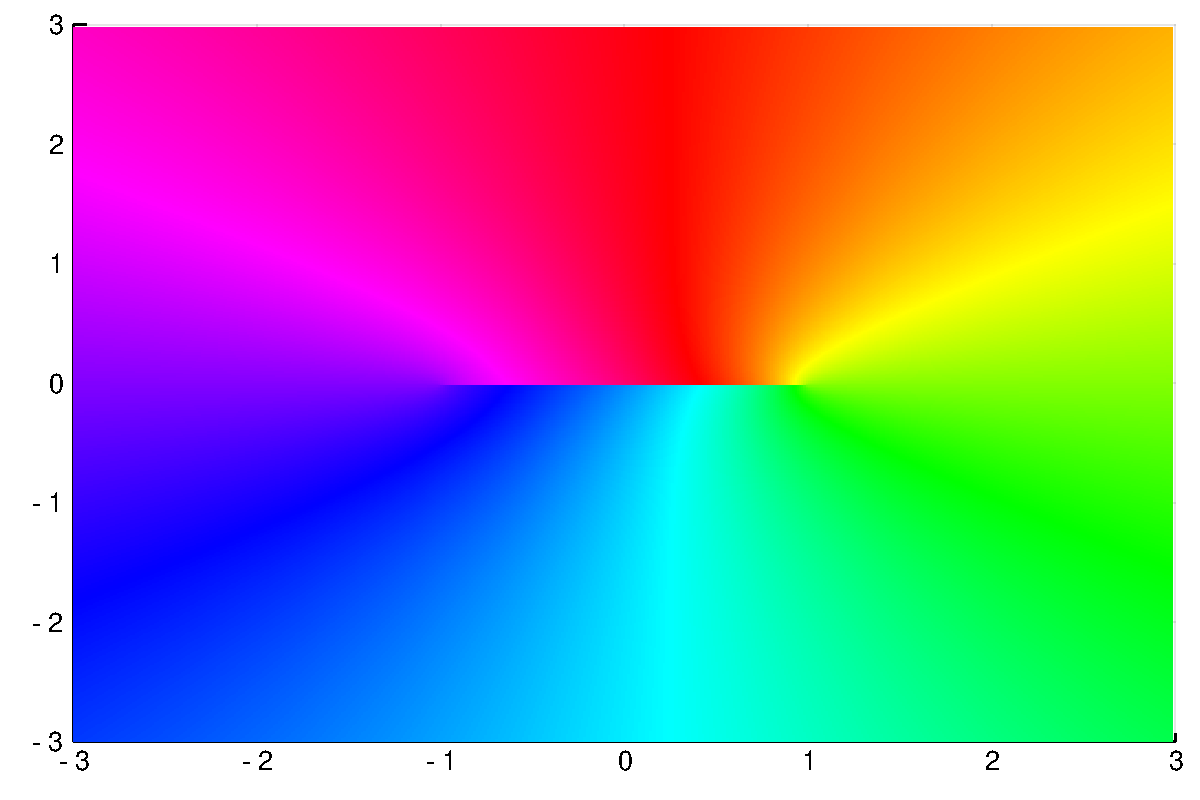
\includegraphics[width=\linewidth]{figures/Lecture12_1_1.pdf}

What's evident here is that it has a jump on the contour.  It turns out that the Cauchy transform has a very simple subtractive jump. Here we denote

\[
    \CC_{[a,b]}^+ f(x) = \lim_{\epsilon \rightarrow 0^+} \CC_{[a,b]} f( x+ \I \epsilon)\\
        \CC_{[a,b]}^- f(x) = \lim_{\epsilon \rightarrow 0^+} \CC_{[a,b]} f( x- \I \epsilon)
\]
that is the limit from above and below. For more complicated contours these would denote limit from the left/right or in the case of a simple closed contour, interior/exterior. 

\textbf{Theorem (Plemelj on the interval I)} Suppose $(b-x)^\alpha (x-a)^\beta f(x)$ is differentiable  on $[a,b]$, for $\alpha, \beta < 1$.  Then the Cauchy transform has the following properties:

\begin{itemize}
\item[1. ] \emph{Analyticity}: $\CC_{[a,b]} f(z)$ is analytic in $\bar \C \backslash [a,b]$


\item[2. ] \emph{Decay}: $\CC_{[a,b]} f(\infty) = 0$


\item[3. ] \emph{Jump}: It has the subtractive jump:

\end{itemize}
\[
\CC_{[a,b]}^+ f(x) - \CC_{[a,b]}^- f(x) = f(x) \qqfor a < x < b
\]
\begin{itemize}
\item[2. ] \emph{Regularity}: $\CC_{[a,b]} f(z)$ has weaker than pole singularities at $a$ and $b$

\end{itemize}
\textbf{Sketch of Proof}  We show the proof for $[-1,1]$.

\begin{itemize}
\item[1. ] From the dominated convergence theorem, we know that $\CC f(z)$ is complex-differentiable off $[-1,1]$:

\end{itemize}
\[
{\D \over \D z} {\cal C} f(z) = {1 \over 2 \pi \I}\int_{-1}^1  {\D \over \D z} {f(x) \over x - z} \dx = {1 \over 2 \pi \I}\int_{-1}^1   {f(x) \over (x - z)^2} \dx
\]
We know it is analytic at $\infty$ because

\[
{\cal C} f(z^{-1}) = z {1 \over 2 \pi \I}\int_{-1}^1   {f(x) \over z x - 1} \dx
\]
is differentiable at zero. 

\begin{itemize}
\item[2. ] \[
{\cal C} f(\infty) = 0
\]
follows from uniform convergence of $1 \over z - x$ to zero as $z \rightarrow \infty$.


\item[3. ] For the constant function, which is analytic, this follows by considering a contour $\gamma_x^+$ perturbed above $x$ and $\gamma_x^-$ perturbed below $x$, see plots below.  Therefore, by Cauchy integral formula we have

\end{itemize}
\[
\CC^+ 1 (x) - \CC^- 1 (x) = {1 \over 2 \pi \I}\int_{\gamma_x^+} {1 \over x - z} \dx - {1 \over 2 \pi \I}\int_{\gamma_x^-} {1 \over x - z} \dx = {1 \over 2 \pi \I} \oint {1 \over x -z } \dx = 1.
\]
For other functions, we consider, for $z = x + \I \epsilon$,

\[
    {\cal C} f(z) =   {1 \over 2 \pi \I} \int_{-1}^1 {f(t) - f(x) \over t - z} \dt + f(x) \CC 1(z)
\]
For $\epsilon = 0$, the first integral exists because the singularity at $t = x$ is removable: 

\[
\lim_{t \rightarrow x} {f(t) - f(x) \over t - x} = f'(x)
\]
We leave it as an excercise (or see [Trogdon \& Olver 2015, Lemma 2.7]) to show that $\int_{-1}^1 {f(t) - f(x) \over t - z} \dt$ converges to $\int_{-1}^1 {f(t) - f(x) \over t - x} \dt$ as $z \rightarrow x$. It follows that

\[
{\cal C}^\pm f(x) =   {1 \over 2 \pi \I} \int_{-1}^1 {f(t) - f(x) \over t - x} \dt + f(x) \CC^\pm 1(x)
\]
and in particular

\[
{\cal C}^+ f(x) - {\cal C}^- f(x)  =  f(x) (\CC^+ 1(x) - \CC^- 1(x)) = f(x)
\]
\begin{itemize}
\item[4. ] We show that it has a weaker than pole singularity at $+1$, with $-1$ following by the same argument. First note that $f$ is absolutely integrable. 

\end{itemize}
If we assume we approach $1$ at an angle of $-\pi + \delta \leq \theta \leq \pi - \delta$, the uniform convergence of $(z - 1) \CC f(z)$ to zero follows from observing that ${z-1 \over z - t}$ can be made arbitrarily small in a larger and larger interval. This is easiest to see for real $x > 1$, where for  $1 \leq x \leq 1 + \epsilon^2$ we have

\[
\left|{x -1 \over x-t }\right| \leq \epsilon
\]
for all $t \leq 1 + \epsilon^2 - \epsilon$, or more generously, $t \leq 1 - \epsilon$. Therefore,

\[
| (x-1) {\cal C} f(x) | \leq {1 \over 2 \pi}\int_{-1}^{1-\epsilon} |f(t) | \left|{x -1 \over x-t }\right| \dt + \int_{1-\epsilon}^1 |f(t) | \dt \leq
\epsilon \int_{-1}^1 |f(t)| \dt + \int_{1-\epsilon}^1 |f(t) | \dt
\]
Both terms tends to zero as $\epsilon \rightarrow 0$, hence so does $| (x-1) {\cal C} f(x) |$.  To extend this to the interval itself (that is, $\delta = 0$), we  use the stronger requirement that $(1-x)^\alpha(1+x)^\beta f(x)$ is differentiable. For $\alpha = \beta = 0$, this follows from the expression in condition (3) and the fact that (found via direct integration)

\[
    \CC 1(z) =  {\log(z-1) - \log(z+1) \over 2 \pi \I}
\]
has only logarithmic singularities, and $f(x)$ is bounded.

\ensuremath{\blacksquare}

Here is a plot of ${x - 1 \over x- t}$ showing that it is small on an increasing portion of the interval as $x \rightarrow 1$ from the right:


\begin{lstlisting}
(*@\HLJLn{x}@*) (*@\HLJLoB{=}@*) (*@\HLJLni{1}@*) (*@\HLJLoB{+}@*) (*@\HLJLnfB{0.01}@*)
(*@\HLJLn{tt}@*) (*@\HLJLoB{=}@*) (*@\HLJLnf{range}@*)(*@\HLJLp{(}@*)(*@\HLJLoB{-}@*)(*@\HLJLnfB{1.}@*)(*@\HLJLp{,}@*)(*@\HLJLnfB{1.}@*)(*@\HLJLp{;}@*) (*@\HLJLn{length}@*)(*@\HLJLoB{=}@*)(*@\HLJLni{1000}@*)(*@\HLJLp{)}@*)
(*@\HLJLnf{plot}@*)(*@\HLJLp{(}@*)(*@\HLJLn{tt}@*)(*@\HLJLp{,}@*) (*@\HLJLn{abs}@*)(*@\HLJLoB{.}@*)(*@\HLJLp{((}@*)(*@\HLJLn{x}@*) (*@\HLJLoB{-}@*) (*@\HLJLni{1}@*)(*@\HLJLp{)}@*) (*@\HLJLoB{./}@*) (*@\HLJLp{(}@*)(*@\HLJLn{x}@*) (*@\HLJLoB{.-}@*) (*@\HLJLn{tt}@*)(*@\HLJLp{));}@*) (*@\HLJLn{legend}@*)(*@\HLJLoB{=}@*)(*@\HLJLkc{false}@*)(*@\HLJLp{)}@*)
\end{lstlisting}

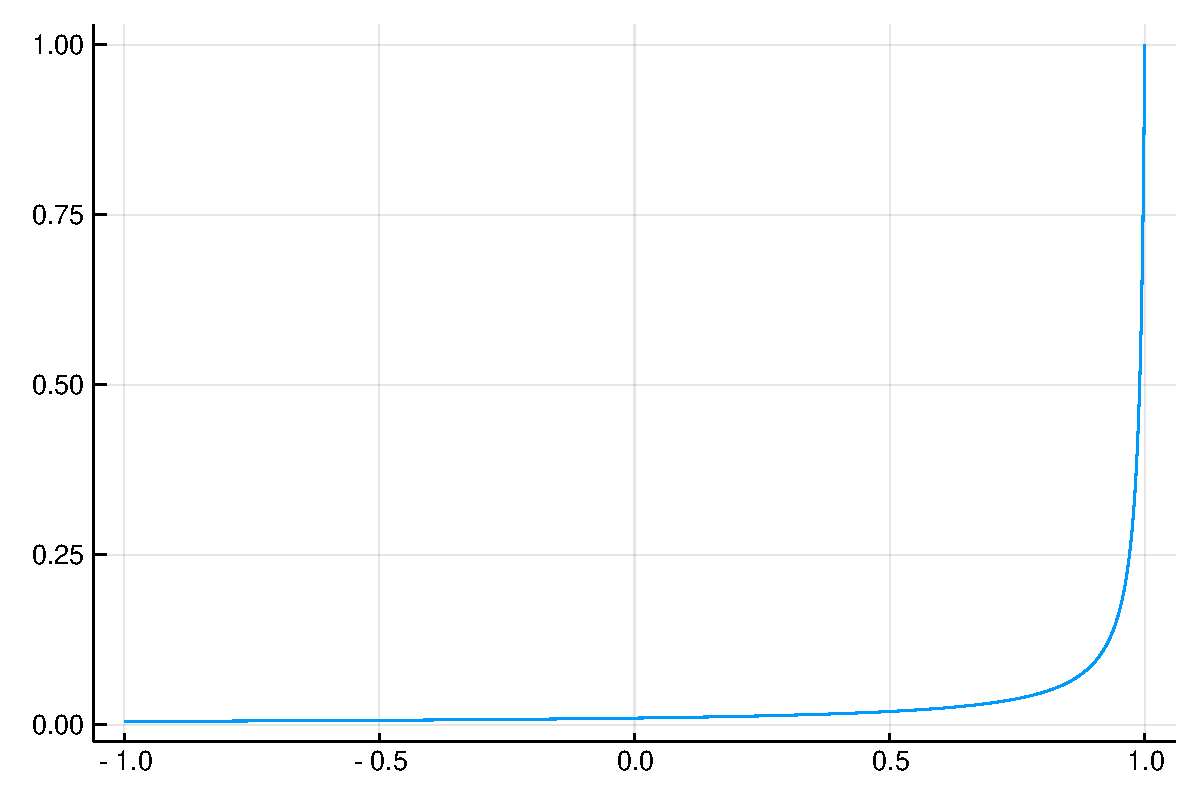
\includegraphics[width=\linewidth]{figures/Lecture12_2_1.pdf}

Here is a plot of $\gamma_x^\pm$:


\begin{lstlisting}
(*@\HLJLn{x}@*) (*@\HLJLoB{=}@*) (*@\HLJLnfB{0.4}@*)
(*@\HLJLn{r}@*) (*@\HLJLoB{=}@*) (*@\HLJLnfB{0.1}@*)
(*@\HLJLn{tt}@*) (*@\HLJLoB{=}@*) (*@\HLJLnf{range}@*)(*@\HLJLp{(}@*)(*@\HLJLn{\ensuremath{\pi}}@*)(*@\HLJLp{,}@*)(*@\HLJLnfB{0.}@*)(*@\HLJLp{;}@*) (*@\HLJLn{length}@*)(*@\HLJLoB{=}@*)(*@\HLJLni{100}@*)(*@\HLJLp{)}@*)
(*@\HLJLnf{plot}@*)(*@\HLJLp{([}@*)(*@\HLJLoB{-}@*)(*@\HLJLnfB{1.}@*)(*@\HLJLp{;}@*) (*@\HLJLn{x}@*) (*@\HLJLoB{.+}@*) (*@\HLJLn{r}@*)(*@\HLJLoB{*}@*)(*@\HLJLn{cos}@*)(*@\HLJLoB{.}@*)(*@\HLJLp{(}@*)(*@\HLJLn{tt}@*)(*@\HLJLp{);}@*)(*@\HLJLnfB{1.0}@*)(*@\HLJLp{],}@*) (*@\HLJLp{[}@*)(*@\HLJLnfB{0.}@*)(*@\HLJLp{;}@*) (*@\HLJLn{r}@*)(*@\HLJLoB{*}@*)(*@\HLJLn{sin}@*)(*@\HLJLoB{.}@*)(*@\HLJLp{(}@*)(*@\HLJLn{tt}@*)(*@\HLJLp{);}@*) (*@\HLJLnfB{0.0}@*)(*@\HLJLp{];}@*)(*@\HLJLn{ylims}@*)(*@\HLJLoB{=}@*)(*@\HLJLp{(}@*)(*@\HLJLoB{-}@*)(*@\HLJLnfB{0.5}@*)(*@\HLJLp{,}@*)(*@\HLJLnfB{0.5}@*)(*@\HLJLp{),}@*)(*@\HLJLn{label}@*)(*@\HLJLoB{=}@*)(*@\HLJLs{"{}g{\_}x{\textasciicircum}+"{}}@*)(*@\HLJLp{)}@*)
(*@\HLJLnf{plot!}@*)(*@\HLJLp{([}@*)(*@\HLJLoB{-}@*)(*@\HLJLnfB{1.}@*)(*@\HLJLp{;}@*) (*@\HLJLn{x}@*) (*@\HLJLoB{.+}@*) (*@\HLJLn{r}@*)(*@\HLJLoB{*}@*)(*@\HLJLn{cos}@*)(*@\HLJLoB{.}@*)(*@\HLJLp{(}@*)(*@\HLJLn{tt}@*)(*@\HLJLp{);}@*)(*@\HLJLnfB{1.0}@*)(*@\HLJLp{],}@*) (*@\HLJLp{[}@*)(*@\HLJLnfB{0.}@*)(*@\HLJLp{;}@*) (*@\HLJLoB{-}@*)(*@\HLJLn{r}@*)(*@\HLJLoB{*}@*)(*@\HLJLn{sin}@*)(*@\HLJLoB{.}@*)(*@\HLJLp{(}@*)(*@\HLJLn{tt}@*)(*@\HLJLp{);}@*) (*@\HLJLnfB{0.0}@*)(*@\HLJLp{];}@*)(*@\HLJLn{ylims}@*)(*@\HLJLoB{=}@*)(*@\HLJLp{(}@*)(*@\HLJLoB{-}@*)(*@\HLJLnfB{0.5}@*)(*@\HLJLp{,}@*)(*@\HLJLnfB{0.5}@*)(*@\HLJLp{),}@*)(*@\HLJLn{label}@*)(*@\HLJLoB{=}@*)(*@\HLJLs{"{}g{\_}x{\textasciicircum}-"{}}@*)(*@\HLJLp{)}@*)
\end{lstlisting}

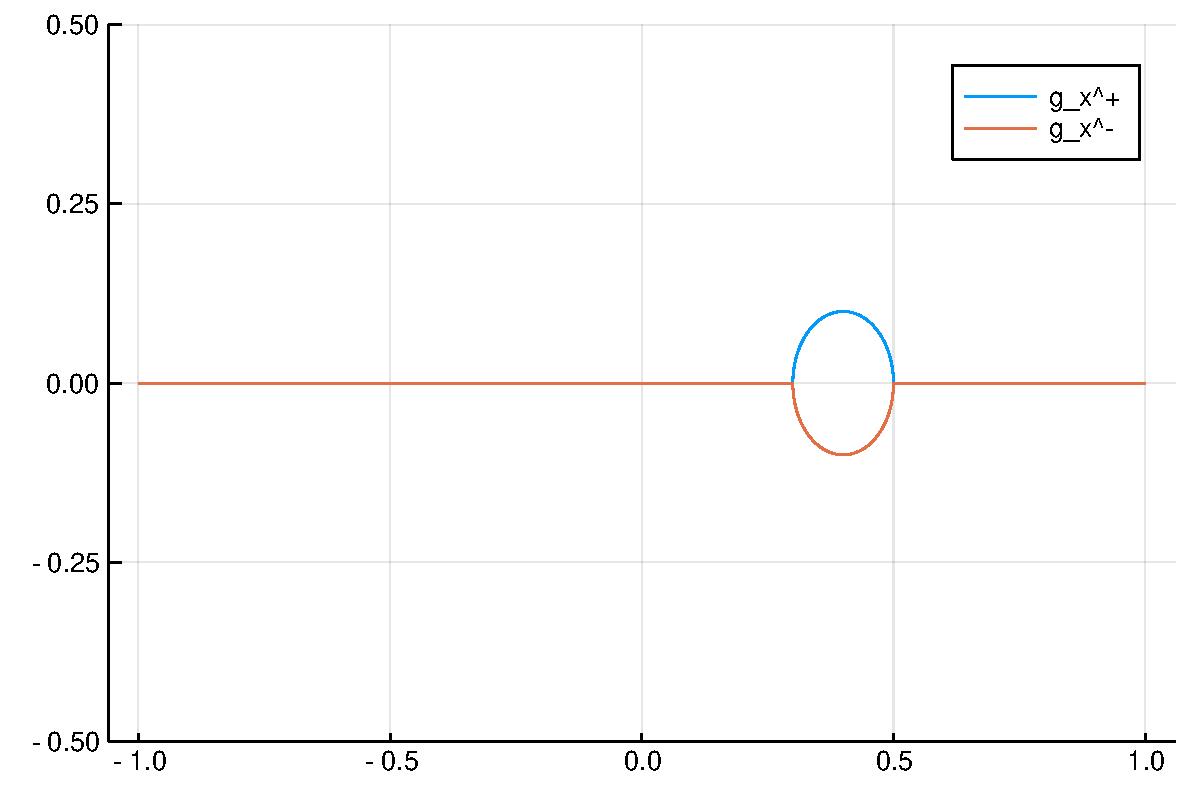
\includegraphics[width=\linewidth]{figures/Lecture12_3_1.pdf}

We can use the results of the previous results to show that it is in fact unique.

\textbf{Theorem (Plemelj on the interval II)} Suppose $\phi(z)$ satsfies the following properties:

\begin{itemize}
\item[1. ] \emph{Analyticity}: $\phi(z)$ is analytic in $\bar \C \backslash [a,b]$


\item[2. ] \emph{Regularity}: $\phi(z)$ has weaker than pole singularities at $a$ and $b$


\item[3. ] \emph{Decay}: $\phi(\infty) = 0$


\item[4. ] \emph{Jump}: It has the subtractive jump:

\end{itemize}
\[
\phi^+(x) - \phi^-(x) = f(x) \qqfor a < x < b
\]
where $(b-x)^\alpha (x-a)^\beta f(x)$ is differentiable in $[a,b]$ for $\alpha,\beta < 1$.  

Then $\phi(z) = {\cal C}_{[a,b]} f(z)$.

\textbf{Sketch of Proof} Consider 

\[
A(z) = \phi(z) - {\cal C}_{[a,b]} f(z)
\]
This is continuous (hence analytic) on $(a,b)$ as

\[
A^+(x) - A^-(x) = \phi^+(x) -\phi^-(x) - {\cal C}_{[a,b]}^+ f(x) + {\cal C}_{[a,b]}^- f(x)  =f(x) - f(x) = 0
\]
Also, $A$ has weaker than pole singularities at $a$ and $b$, hence is analytic there as well: it's entire.  Only entire functions that are bounded are constant, since it vanishes at $\infty$ the constant must be zero.

\ensuremath{\blacksquare}

\emph{Example 1} We can use this theorem to prove the following relationships  (using $\diamond$ for the dummy variable):

\[
{1 \over \sqrt{z-1} \sqrt{z+1}} = -2 \I {\cal C}\left[{1 \over \sqrt{1-\diamond^2}}\right](z) = 
-{1 \over \pi}\int_{-1}^1 {\dx \over \sqrt{1-x^2} (x-z)}
\]
(1) follows because the jumps cancel. (2 and 3) are immediate. (4) follows from a simple calculation.  Here we show that it has the correct jump:


\begin{lstlisting}
(*@\HLJLn{x}@*) (*@\HLJLoB{=}@*) (*@\HLJLnf{Fun}@*)(*@\HLJLp{()}@*)
(*@\HLJLn{z}@*) (*@\HLJLoB{=}@*) (*@\HLJLni{2}@*) (*@\HLJLoB{+}@*)(*@\HLJLni{2}@*)(*@\HLJLn{im}@*)
(*@\HLJLni{1}@*)(*@\HLJLoB{/}@*)(*@\HLJLp{(}@*)(*@\HLJLnf{sqrt}@*)(*@\HLJLp{(}@*)(*@\HLJLn{z}@*)(*@\HLJLoB{-}@*)(*@\HLJLni{1}@*)(*@\HLJLp{)}@*)(*@\HLJLnf{sqrt}@*)(*@\HLJLp{(}@*)(*@\HLJLn{z}@*)(*@\HLJLoB{+}@*)(*@\HLJLni{1}@*)(*@\HLJLp{)),}@*)(*@\HLJLoB{-}@*)(*@\HLJLni{2}@*)(*@\HLJLn{im}@*)(*@\HLJLoB{*}@*)(*@\HLJLnf{cauchy}@*)(*@\HLJLp{(}@*)(*@\HLJLni{1}@*)(*@\HLJLoB{/}@*)(*@\HLJLnf{sqrt}@*)(*@\HLJLp{(}@*)(*@\HLJLni{1}@*)(*@\HLJLoB{-}@*)(*@\HLJLn{x}@*)(*@\HLJLoB{{\textasciicircum}}@*)(*@\HLJLni{2}@*)(*@\HLJLp{),}@*)(*@\HLJLn{z}@*)(*@\HLJLp{)}@*)
\end{lstlisting}

\begin{lstlisting}
(0.23307736827563616 - 0.2640258983261148im, 0.2330773682756362 - 0.2640258
983261148im)
\end{lstlisting}


\emph{Example 2} Now consider a problem of reducing 

\[
\phi(z) = \sqrt{z-1} \sqrt{z+1}
\]
to its behaviour near its singularities. It has two singularities: it blows up at $\infty$ and has a branch cut on $[-1,1]$

We can subtract out the singularity at infinity first to determine

\[
\phi(z) = z  + 2 \I {\cal C}[\sqrt{1-\diamond^2}](z)
\]
Note this works because, as $z \rightarrow \infty$, we have 

\[
\phi(z) = z (\sqrt{1-{1/z}}\sqrt{1 + {1/z}}) = z (1 + O({1/z}))(1+O(1/z)) = z + O(1/z)
\]
hence $\phi(z) - z$ vanishes at the origin. This is an example of summing over the behaviour at each singularity to  recover the function (in this case, $\phi$ has a singularity along the cut $[-1,1]$ and polynomial growth at $\infty$). 

Because $\phi(z)-z$ decays, we can now deploy Plemelj II to determine:

\[
\phi(z) -z = \CC[\phi_+-\phi_-](z)
\]
where

\[
\phi_+(x) - \phi_-(x) = 2\I \sqrt{1-x^2}
\]
Here we see that our derived expression matches $phi(z)$:


\begin{lstlisting}
(*@\HLJLnf{sqrt}@*)(*@\HLJLp{(}@*)(*@\HLJLn{z}@*)(*@\HLJLoB{-}@*)(*@\HLJLni{1}@*)(*@\HLJLp{)}@*)(*@\HLJLnf{sqrt}@*)(*@\HLJLp{(}@*)(*@\HLJLn{z}@*)(*@\HLJLoB{+}@*)(*@\HLJLni{1}@*)(*@\HLJLp{),}@*) (*@\HLJLn{z}@*) (*@\HLJLoB{+}@*)(*@\HLJLni{2}@*)(*@\HLJLn{im}@*)(*@\HLJLoB{*}@*)(*@\HLJLnf{cauchy}@*)(*@\HLJLp{(}@*)(*@\HLJLnf{sqrt}@*)(*@\HLJLp{(}@*)(*@\HLJLni{1}@*)(*@\HLJLoB{-}@*)(*@\HLJLn{x}@*)(*@\HLJLoB{{\textasciicircum}}@*)(*@\HLJLni{2}@*)(*@\HLJLp{),}@*)(*@\HLJLn{z}@*)(*@\HLJLp{)}@*)
\end{lstlisting}

\begin{lstlisting}
(1.8791298183332827 + 2.1286448445312045im, 1.8791298183332823 + 2.12864484
4531204im)
\end{lstlisting}


\emph{Example 3} Finally, we have the following (also verifiable using indefinite integration):

\[
{\log(z-1) - \log(z+1) \over 2 \pi \I} =  {\cal C}[1](z) = {1 \over 2 \pi \I} \int_{-1}^1 {\dx \over x -z}
\]

\begin{lstlisting}
(*@\HLJLp{(}@*)(*@\HLJLnf{log}@*)(*@\HLJLp{(}@*)(*@\HLJLn{z}@*)(*@\HLJLoB{-}@*)(*@\HLJLni{1}@*)(*@\HLJLp{)}@*)(*@\HLJLoB{-}@*)(*@\HLJLnf{log}@*)(*@\HLJLp{(}@*)(*@\HLJLn{z}@*)(*@\HLJLoB{+}@*)(*@\HLJLni{1}@*)(*@\HLJLp{))}@*)(*@\HLJLoB{/}@*)(*@\HLJLp{(}@*)(*@\HLJLni{2}@*)(*@\HLJLn{\ensuremath{\pi}}@*)(*@\HLJLoB{*}@*)(*@\HLJLn{im}@*)(*@\HLJLp{),}@*)(*@\HLJLnf{cauchy}@*)(*@\HLJLp{(}@*)(*@\HLJLnf{Fun}@*)(*@\HLJLp{(}@*)(*@\HLJLnf{one}@*)(*@\HLJLp{(}@*)(*@\HLJLn{x}@*)(*@\HLJLp{)),}@*)(*@\HLJLn{z}@*)(*@\HLJLp{)}@*)
\end{lstlisting}

\begin{lstlisting}
(0.08262467026928395 + 0.07603718482849817im, 0.08262467026928397 + 0.07603
718482849817im)
\end{lstlisting}


\subsubsection{Uniqueness results from inferred singularity}
Recall that an important ingredient of complex analysis is Liouville's theorem:

\textbf{Theorem (Liouville)} If $f$ is entire and  bounded in ${\mathbb C}$, then $f$ must be constant.

We will see that knowledge of the behaviour of $\phi$ can be used to recover by its behaviour at  its singularities at $\infty$ and jump on $[-1,1]$. But before that, we already have the following  uniqueness results by combining the above with Liouville's theorem:

\begin{itemize}
\item[1. ] \[
\phi(z)
\]
is the unique function analytic in $\C \backslash [-1,1]$ with weaker than pole singularities at $\pm 1$ satisfying $\phi(z) \sim z$ and 

\end{itemize}
\[
\phi_+(x) - \phi_-(x) = 2\I \sqrt{1-x^2} \qqfor -1 < x <1.
\]
\begin{itemize}
\item[2. ] \[
\kappa(z) = {1 \over \sqrt{z-1} \sqrt{z+1}}
\]
is the unique function analytic in $\bar\C \backslash [-1,1]$ with weaker than pole singularities at $\pm 1$ satisfying $\kappa(\infty) = 0$ and 

\end{itemize}
\[
\kappa_+(x) - \kappa_-(x) = {-2\I \over \sqrt{1-x^2}}\qqfor -1 < x <1.
\]
\emph{Demonstration} From the phase plot we see it has a branch cut on $[-1,1]$:


\begin{lstlisting}
(*@\HLJLn{\ensuremath{\kappa}}@*) (*@\HLJLoB{=}@*) (*@\HLJLn{z}@*) (*@\HLJLoB{->}@*) (*@\HLJLni{1}@*)(*@\HLJLoB{/}@*)(*@\HLJLp{(}@*)(*@\HLJLnf{sqrt}@*)(*@\HLJLp{(}@*)(*@\HLJLn{z}@*)(*@\HLJLoB{-}@*)(*@\HLJLni{1}@*)(*@\HLJLp{)}@*)(*@\HLJLnf{sqrt}@*)(*@\HLJLp{(}@*)(*@\HLJLn{z}@*)(*@\HLJLoB{+}@*)(*@\HLJLni{1}@*)(*@\HLJLp{))}@*)
(*@\HLJLnf{phaseplot}@*)(*@\HLJLp{(}@*)(*@\HLJLoB{-}@*)(*@\HLJLnfB{3..3}@*)(*@\HLJLp{,}@*) (*@\HLJLoB{-}@*)(*@\HLJLnfB{3..3}@*)(*@\HLJLp{,}@*) (*@\HLJLn{\ensuremath{\kappa}}@*)(*@\HLJLp{)}@*)
\end{lstlisting}

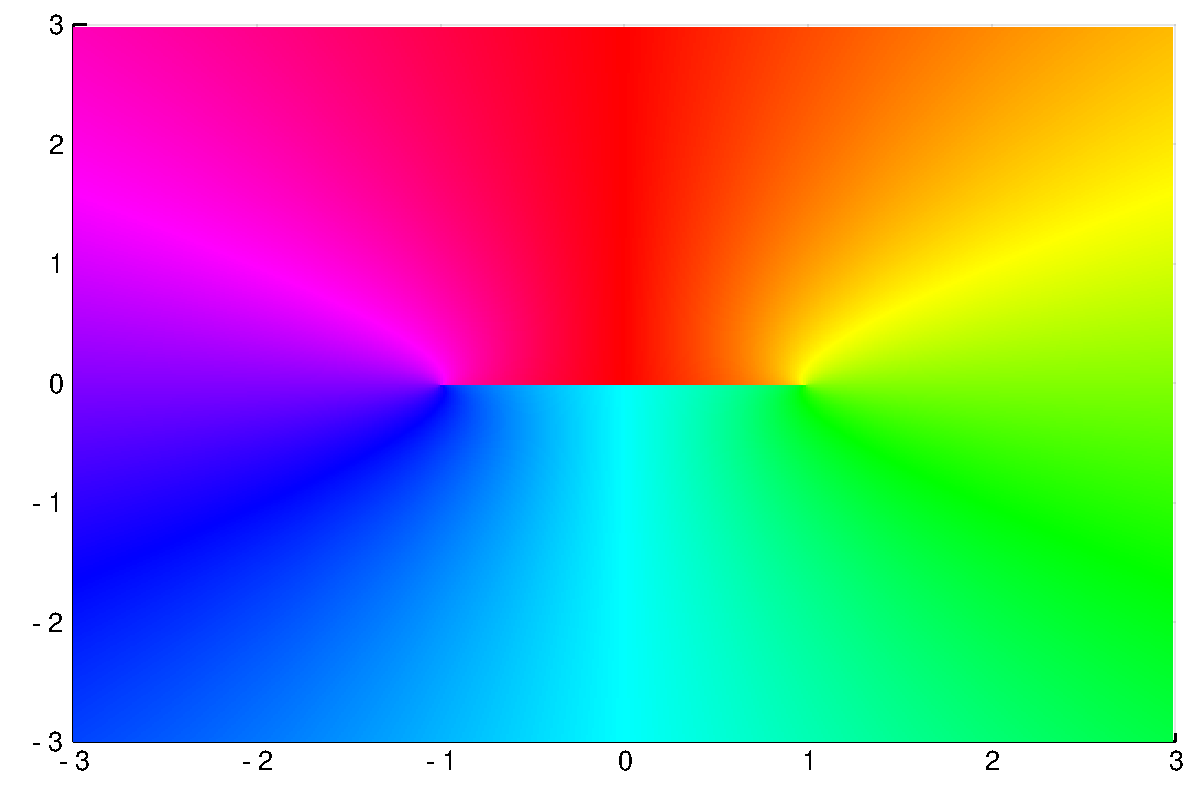
\includegraphics[width=\linewidth]{figures/Lecture12_7_1.pdf}

On the branch there is the expected jump:


\begin{lstlisting}
(*@\HLJLn{x}@*) (*@\HLJLoB{=}@*) (*@\HLJLnfB{0.1}@*)
(*@\HLJLnf{\ensuremath{\kappa}}@*)(*@\HLJLp{(}@*)(*@\HLJLn{x}@*) (*@\HLJLoB{+}@*) (*@\HLJLnfB{0.0}@*)(*@\HLJLn{im}@*)(*@\HLJLp{)}@*) (*@\HLJLoB{-}@*) (*@\HLJLnf{\ensuremath{\kappa}}@*)(*@\HLJLp{(}@*)(*@\HLJLn{x}@*) (*@\HLJLoB{-}@*) (*@\HLJLnfB{0.0}@*)(*@\HLJLn{im}@*)(*@\HLJLp{)}@*) (*@\HLJLp{,}@*) (*@\HLJLoB{-}@*)(*@\HLJLni{2}@*)(*@\HLJLn{im}@*)(*@\HLJLoB{/}@*)(*@\HLJLnf{sqrt}@*)(*@\HLJLp{(}@*)(*@\HLJLni{1}@*)(*@\HLJLoB{-}@*)(*@\HLJLn{x}@*)(*@\HLJLoB{{\textasciicircum}}@*)(*@\HLJLni{2}@*)(*@\HLJLp{)}@*)
\end{lstlisting}

\begin{lstlisting}
(0.0 - 2.010075630518424im, 0.0 - 2.010075630518424im)
\end{lstlisting}


For $x < -1$ the branch cut is removable: we have continuity and therefore analyticity:


\begin{lstlisting}
(*@\HLJLn{x}@*) (*@\HLJLoB{=}@*) (*@\HLJLoB{-}@*)(*@\HLJLnfB{2.3}@*)
(*@\HLJLnf{\ensuremath{\kappa}}@*)(*@\HLJLp{(}@*)(*@\HLJLn{x}@*) (*@\HLJLoB{+}@*) (*@\HLJLnfB{0.0}@*)(*@\HLJLn{im}@*)(*@\HLJLp{)}@*) (*@\HLJLoB{-}@*) (*@\HLJLnf{\ensuremath{\kappa}}@*)(*@\HLJLp{(}@*)(*@\HLJLn{x}@*) (*@\HLJLoB{-}@*) (*@\HLJLnfB{0.0}@*)(*@\HLJLn{im}@*)(*@\HLJLp{)}@*)
\end{lstlisting}

\begin{lstlisting}
0.0 - 0.0im
\end{lstlisting}


3. $\mu(z) = {\log(z -1) - \log(z+1) \over 2 \pi \I}$ is the unique function analytic in $\C \backslash [-1,1]$ with weaker than pole singularities at $\pm 1$ satisfying $\mu(\infty) = 0$ and 

\[
\mu_+(x) - \mu_-(x) = 1 \qqfor -1 < x < 1.
\]
\emph{Demonstration} Here we see from the phase plot of $mu$ that it has a branch cut on $[-1,1]$:


\begin{lstlisting}
(*@\HLJLn{\ensuremath{\mu}}@*) (*@\HLJLoB{=}@*) (*@\HLJLn{z}@*) (*@\HLJLoB{->}@*) (*@\HLJLp{(}@*)(*@\HLJLnf{log}@*)(*@\HLJLp{(}@*)(*@\HLJLn{z}@*)(*@\HLJLoB{-}@*)(*@\HLJLni{1}@*)(*@\HLJLp{)}@*) (*@\HLJLoB{-}@*) (*@\HLJLnf{log}@*)(*@\HLJLp{(}@*)(*@\HLJLn{z}@*)(*@\HLJLoB{+}@*)(*@\HLJLni{1}@*)(*@\HLJLp{))}@*)(*@\HLJLoB{/}@*)(*@\HLJLp{(}@*)(*@\HLJLni{2}@*)(*@\HLJLn{\ensuremath{\pi}}@*)(*@\HLJLoB{*}@*)(*@\HLJLn{im}@*)(*@\HLJLp{)}@*)
(*@\HLJLnf{phaseplot}@*)(*@\HLJLp{(}@*)(*@\HLJLoB{-}@*)(*@\HLJLnfB{3..3}@*)(*@\HLJLp{,}@*) (*@\HLJLoB{-}@*)(*@\HLJLnfB{3..3}@*)(*@\HLJLp{,}@*) (*@\HLJLn{\ensuremath{\mu}}@*)(*@\HLJLp{)}@*)
\end{lstlisting}

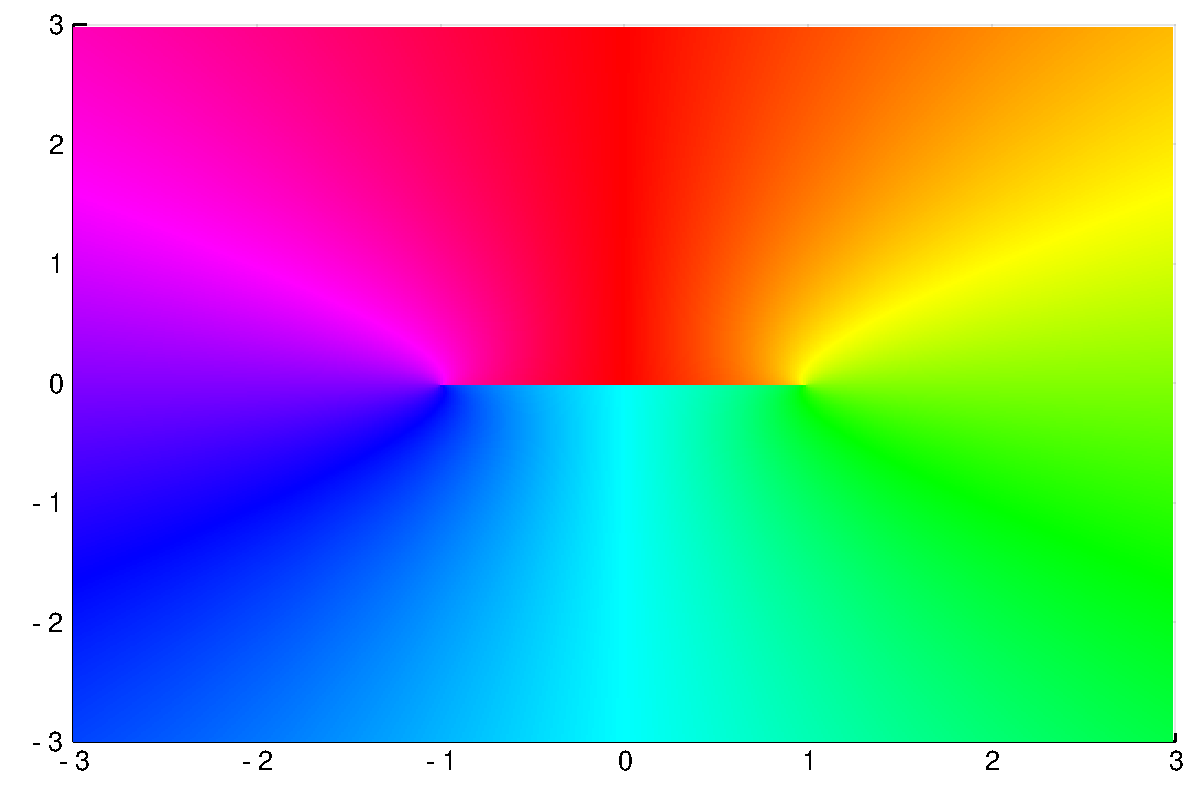
\includegraphics[width=\linewidth]{figures/Lecture12_10_1.pdf}

For $-1 < x < 1$ we have the jump $1$:


\begin{lstlisting}
(*@\HLJLn{x}@*) (*@\HLJLoB{=}@*) (*@\HLJLnfB{0.3}@*)
(*@\HLJLnf{\ensuremath{\mu}}@*)(*@\HLJLp{(}@*)(*@\HLJLn{x}@*) (*@\HLJLoB{+}@*) (*@\HLJLnfB{0.0}@*)(*@\HLJLn{im}@*)(*@\HLJLp{)}@*) (*@\HLJLoB{-}@*) (*@\HLJLnf{\ensuremath{\mu}}@*)(*@\HLJLp{(}@*)(*@\HLJLn{x}@*) (*@\HLJLoB{-}@*) (*@\HLJLnfB{0.0}@*)(*@\HLJLn{im}@*)(*@\HLJLp{)}@*)
\end{lstlisting}

\begin{lstlisting}
1.0 + 0.0im
\end{lstlisting}


For $x < -1$ we see that the branch cuts cancel and we have continuity:


\begin{lstlisting}
(*@\HLJLn{x}@*) (*@\HLJLoB{=}@*) (*@\HLJLoB{-}@*)(*@\HLJLnfB{4.3}@*)
(*@\HLJLnf{\ensuremath{\mu}}@*)(*@\HLJLp{(}@*)(*@\HLJLn{x}@*) (*@\HLJLoB{+}@*) (*@\HLJLnfB{0.0}@*)(*@\HLJLn{im}@*)(*@\HLJLp{)}@*) (*@\HLJLoB{-}@*) (*@\HLJLnf{\ensuremath{\mu}}@*)(*@\HLJLp{(}@*)(*@\HLJLn{x}@*) (*@\HLJLoB{-}@*) (*@\HLJLnfB{0.0}@*)(*@\HLJLn{im}@*)(*@\HLJLp{)}@*)
\end{lstlisting}

\begin{lstlisting}
0.0 + 0.0im
\end{lstlisting}


\textbf{Remark} As an aside, these integrals are computationally difficult because of the singularity in the integrand,  hence standard integration methods become slow as $z$ approaches the interval.  There are other specialised routines (as implemented in \texttt{cauchy(f,z)}) that are much more efficient:


\begin{lstlisting}
(*@\HLJLk{using}@*) (*@\HLJLn{BenchmarkTools}@*)
(*@\HLJLn{z}@*) (*@\HLJLoB{=}@*) (*@\HLJLnfB{0.1}@*) (*@\HLJLoB{+}@*)(*@\HLJLnfB{0.001}@*)(*@\HLJLn{im}@*)
(*@\HLJLnd{@btime}@*) (*@\HLJLnf{cauchy}@*)(*@\HLJLp{(}@*)(*@\HLJLn{f}@*)(*@\HLJLp{,}@*) (*@\HLJLn{z}@*) (*@\HLJLp{)}@*)
\end{lstlisting}

\begin{lstlisting}
494.284 ns (10 allocations: 512 bytes)
\end{lstlisting}


\begin{lstlisting}
(*@\HLJLnd{@btime}@*) (*@\HLJLnf{sum}@*)(*@\HLJLp{(}@*)(*@\HLJLn{f}@*)(*@\HLJLoB{/}@*)(*@\HLJLp{(}@*)(*@\HLJLn{x}@*)(*@\HLJLoB{-}@*)(*@\HLJLn{z}@*)(*@\HLJLp{))}@*)(*@\HLJLoB{/}@*)(*@\HLJLp{(}@*)(*@\HLJLni{2}@*)(*@\HLJLn{\ensuremath{\pi}}@*)(*@\HLJLoB{*}@*)(*@\HLJLn{im}@*)(*@\HLJLp{)}@*)
\end{lstlisting}

\begin{lstlisting}
601.203 ns (6 allocations: 544 bytes)
1.4596050485547113e-5 + 0.06422262213640728im
\end{lstlisting}


We can evaluate the limit from above and below. Here we see numerically that we recover $f$ from taking the difference:


\begin{lstlisting}
(*@\HLJLnf{cauchy}@*)(*@\HLJLp{(}@*)(*@\HLJLn{f}@*)(*@\HLJLp{,}@*) (*@\HLJLnfB{0.1}@*)(*@\HLJLoB{+}@*)(*@\HLJLnfB{0.0}@*)(*@\HLJLn{im}@*)(*@\HLJLp{)}@*)(*@\HLJLoB{-}@*)(*@\HLJLnf{cauchy}@*)(*@\HLJLp{(}@*)(*@\HLJLn{f}@*)(*@\HLJLp{,}@*) (*@\HLJLnfB{0.1}@*)(*@\HLJLoB{-}@*)(*@\HLJLnfB{0.0}@*)(*@\HLJLn{im}@*)(*@\HLJLp{)}@*) (*@\HLJLp{,}@*) (*@\HLJLnf{f}@*)(*@\HLJLp{(}@*)(*@\HLJLnfB{0.1}@*)(*@\HLJLp{)}@*)
\end{lstlisting}

\begin{lstlisting}
(1.0996311793408586 + 0.0im, 1.0996311793408586)
\end{lstlisting}



\end{document}
